\documentclass[a4paper]{article}
\usepackage[utf8]{inputenc}
\usepackage[spanish, es-tabla, es-noshorthands]{babel}
\usepackage[table,xcdraw]{xcolor}
\usepackage[a4paper, footnotesep = 1cm, width=20cm, top=2.5cm, height=25cm, textwidth=18cm, textheight=25cm]{geometry}
%\geometry{showframe}

\usepackage{tikz}
\usepackage{amsmath}
\usepackage{amsfonts}
\usepackage{amssymb}
\usepackage{float}
\usepackage{graphicx}
\usepackage{caption}
\usepackage{subcaption}
\usepackage{multicol}
\usepackage{multirow}
\setlength{\doublerulesep}{\arrayrulewidth}
\usepackage{booktabs}

\usepackage{hyperref}
\hypersetup{
    colorlinks=true,
    linkcolor=blue,
    filecolor=magenta,      
    urlcolor=blue,
    citecolor=blue,    
}

\newcommand{\quotes}[1]{``#1''}
\usepackage{array}
\newcolumntype{C}[1]{>{\centering\let\newline\\\arraybackslash\hspace{0pt}}m{#1}}
\usepackage[american]{circuitikz}
\usetikzlibrary{calc}
\usepackage{fancyhdr}
\usepackage{units} 

\graphicspath{{../Calculos-Potencia/}{../Caracteristicas/}{../Consideraciones/}{../Gain-Stage/}{../Input-Stage/}{../Output-Stage/}{../Simulaciones/}{../Alimentacion/}{../Conclusiones/}}

\pagestyle{fancy}
\fancyhf{}
\lhead{22.12 Electrónica II}
\rhead{Mechoulam, Lambertucci, Rodriguez, Londero, Scala}
\rfoot{Página \thepage}

\begin{document}	

Se consiguió elaborar un amplificador para una carga nominal de $8 \ \Omega$, con una disipación máxima de $1.5 \ kW$ y una distorsión armónica no mayor a $0.529\%$. Es por ello que cabe preguntarse, ¿es posible mejorar el circuito?. Desde nuestro punto de vista, se llegó a la conclusión de que sí se puede mejorar ciertos parámetros, como por ejemplo, la distorsión armónica. La mejora propuesta consiste en el uso de amplificadores operacionales dentro del circuito. Estos permiten reducir el TDH a $0.015 \%$. Otra ventaja que presenta esta implementación es que se puede aplicar una realimentación negativa diferencial mediante el uso de la configuración sumador-restador. Este tipo de realimentación permite subir ..

\begin{figure}[H]
\centering
	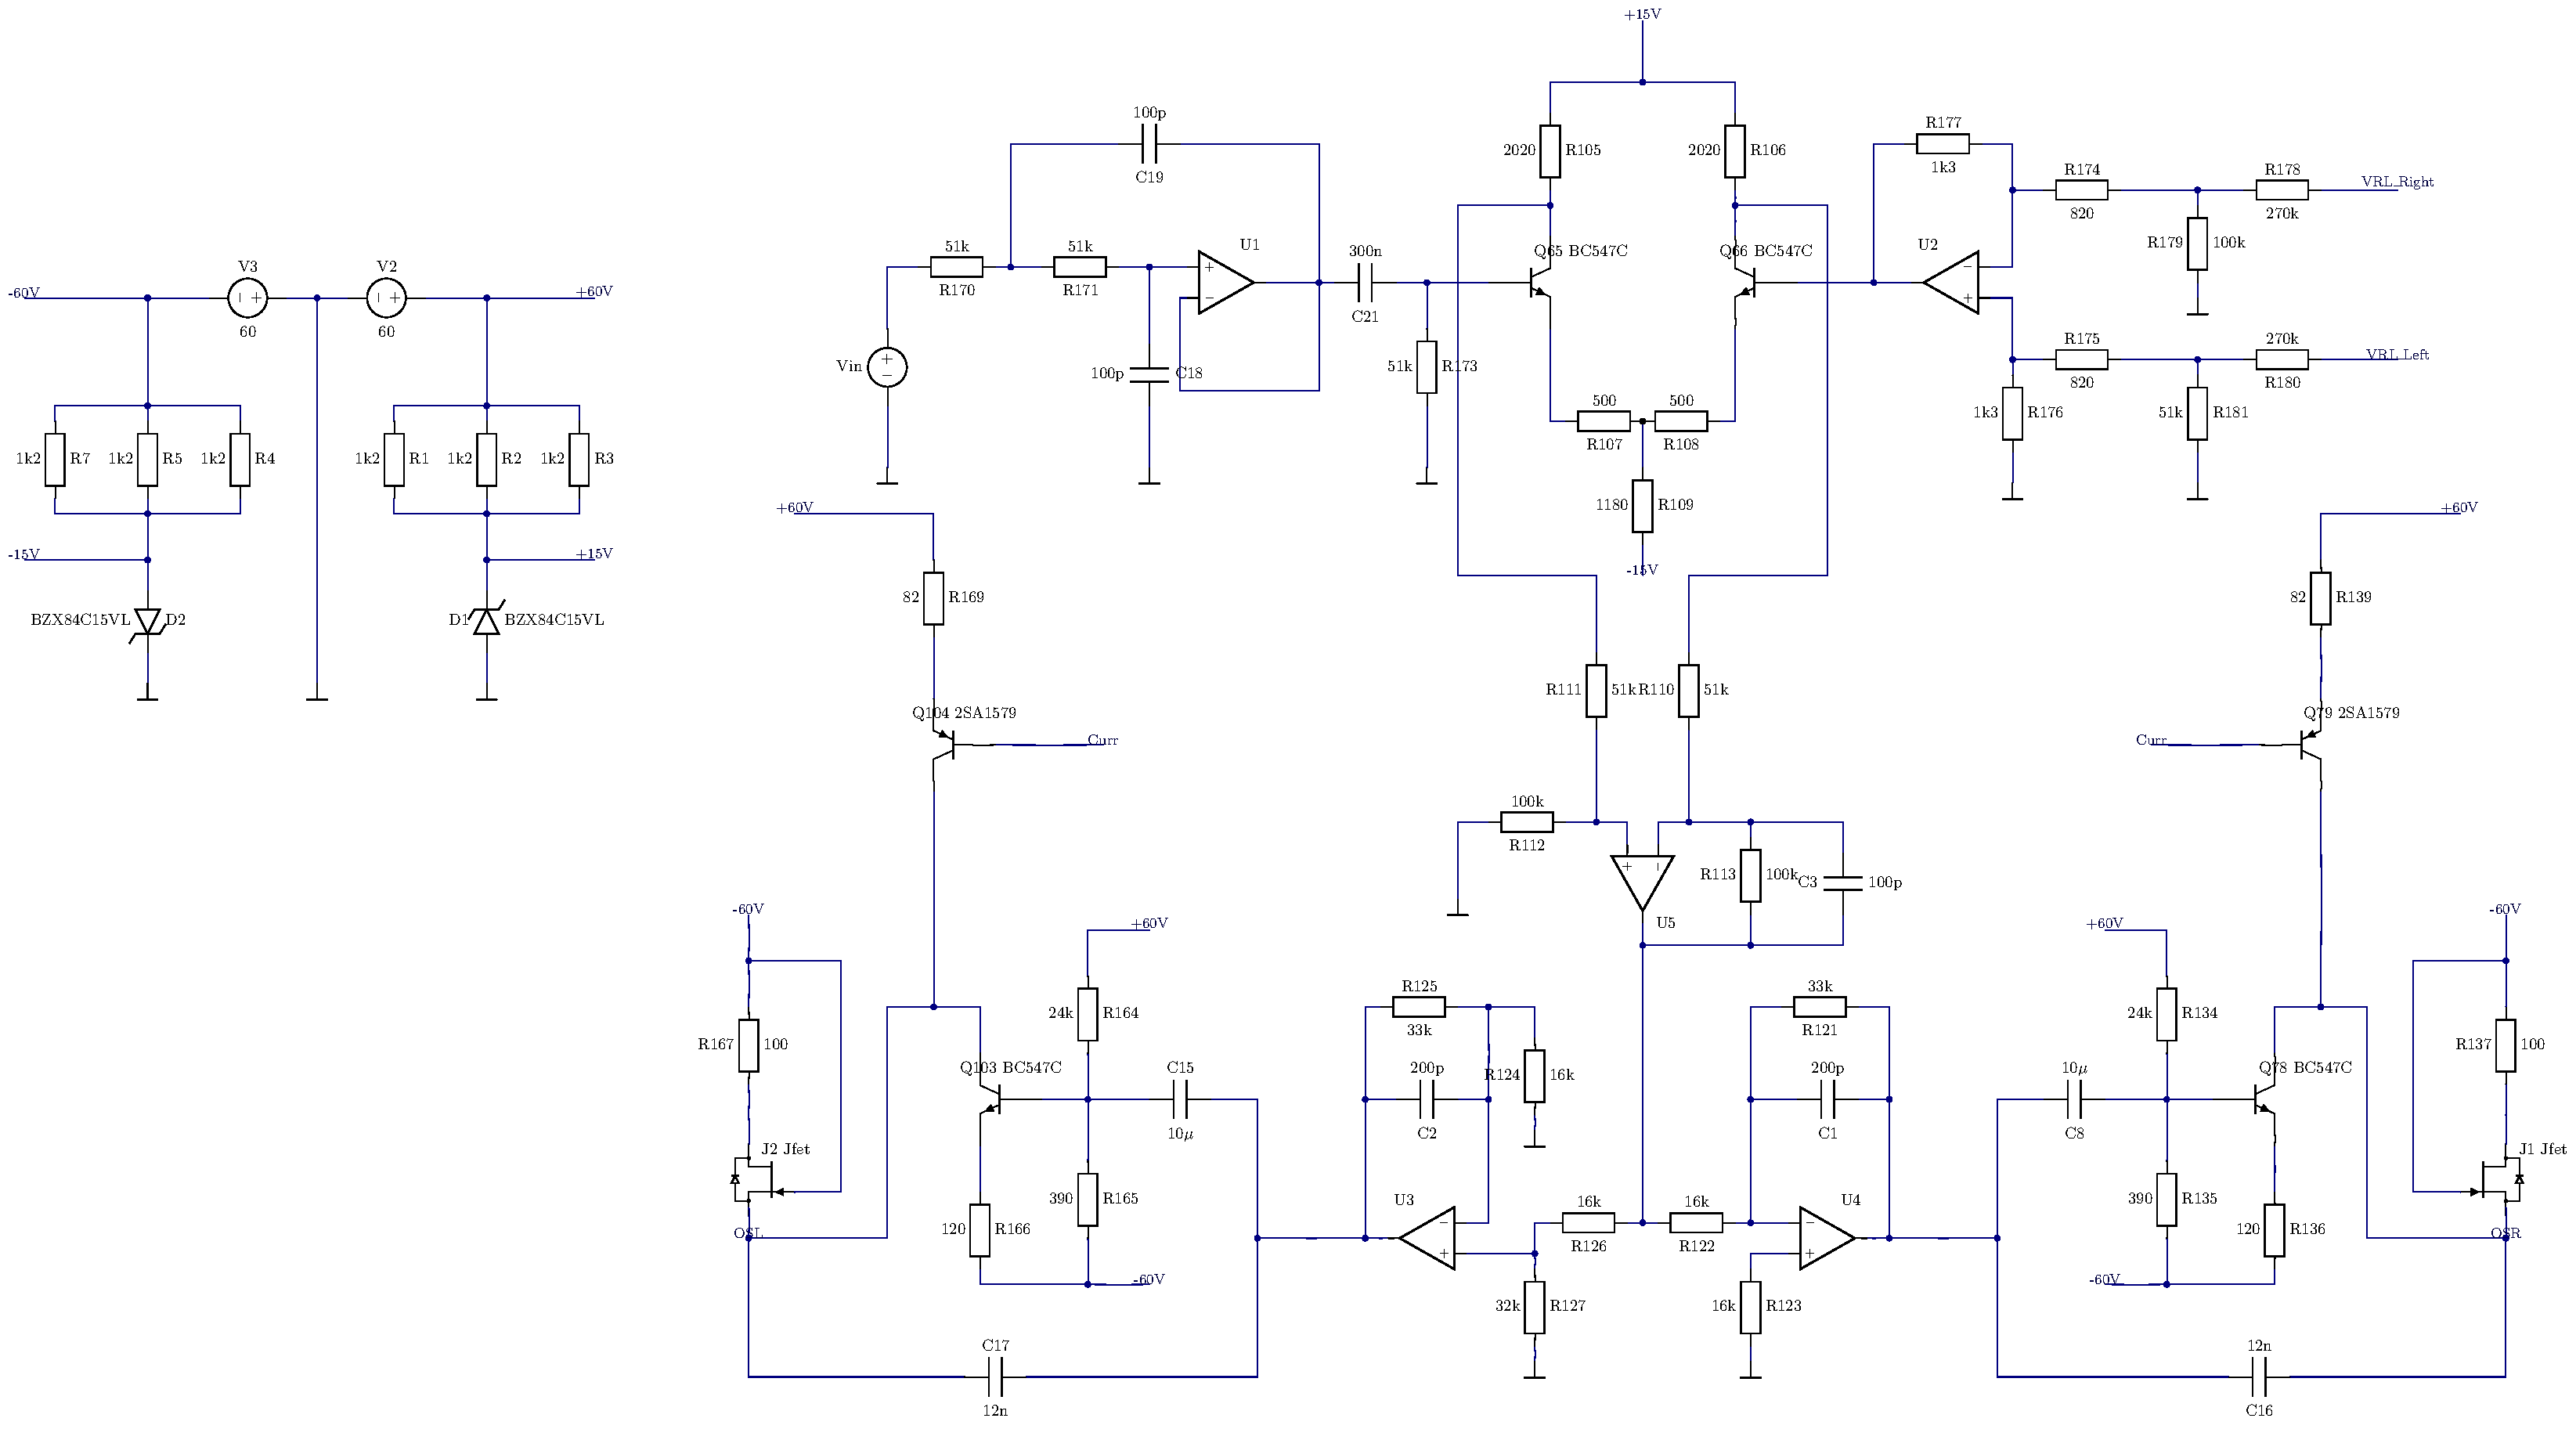
\includegraphics[width=\textwidth]{./ImagenesConclusiones/VOPTEX1.pdf}
	\caption{Etapas de entrada y amplificación (imagen vectorizada la cual no se pixelea).}	
\end{figure}
\begin{figure}[H]
\centering
	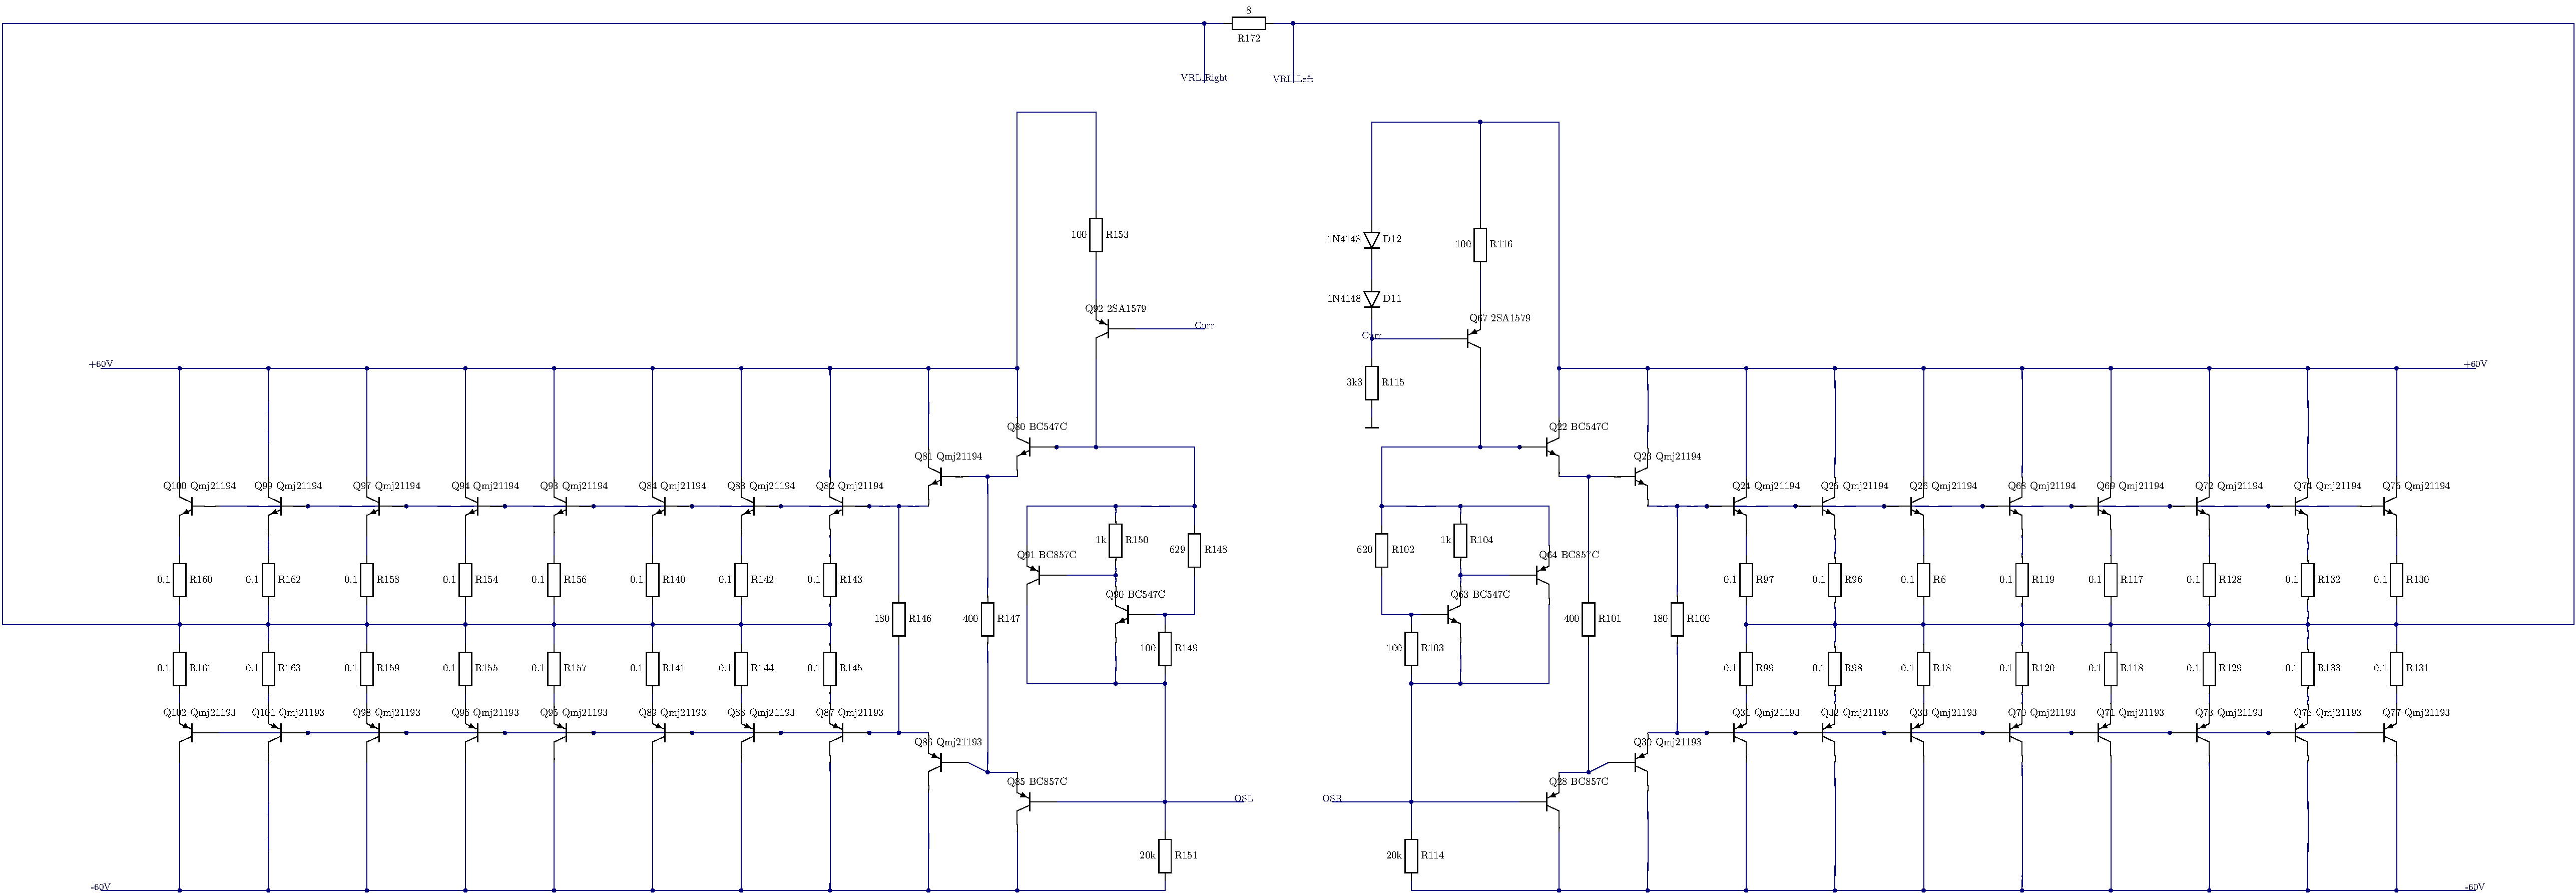
\includegraphics[width=\textwidth]{./ImagenesConclusiones/VOPTEX2.pdf}
	\caption{Etapas de entrada y amplificación (imagen vectorizada la cual no se pixelea).}
\end{figure}

\end{document}